%
% TEXTOS SOBRE O PENSAMENTO MUSICAL
% ---------------------------------
% Agustín de Hipona (San Agustín)
%
\begin{multicols}{2}
%
\subsection*{Pensadores e textos}\label{pensadores-textos}
%
\paragraph{\texorpdfstring{Agustín de Hipona (354-430), \emph{Comentarios
aos salmos}}{Agustín de Hipona (354-430), Comentarios aos salmos}}\label{agustuxedn-de-hipona-354-430--comentarios-aos-salmos}
%
%
Agustín de Hipona é un dos denominados «Pais da Igrexa», é dicir, os primeiros pensadores que desenvolveron nos seus escritos a filosofía do cristianismo. Naceu en Tagaste ( Alxeria) e estudou en Cartago. Inicialmente pagán, converteuse ao cristianismo durante a súa estancia en Milán, onde coñeceu ao bispo Ambrosio; el mesmo chegou a ser bispo de Hipona (Alxeria). Foi canonizado pola igrexa católica. 
Nos seus numerosos escritos hai constantes referencias á música; mesmo escribiu un tratado completo, \emph{De musica}, do que só se conserva unha parte. O seguinte texto, defende e aconsella o uso da música nos cantos relixiosos, fronte á opinión xeral dos bispos da súa época.
%
%\begin{figure}[h]
%\centering
%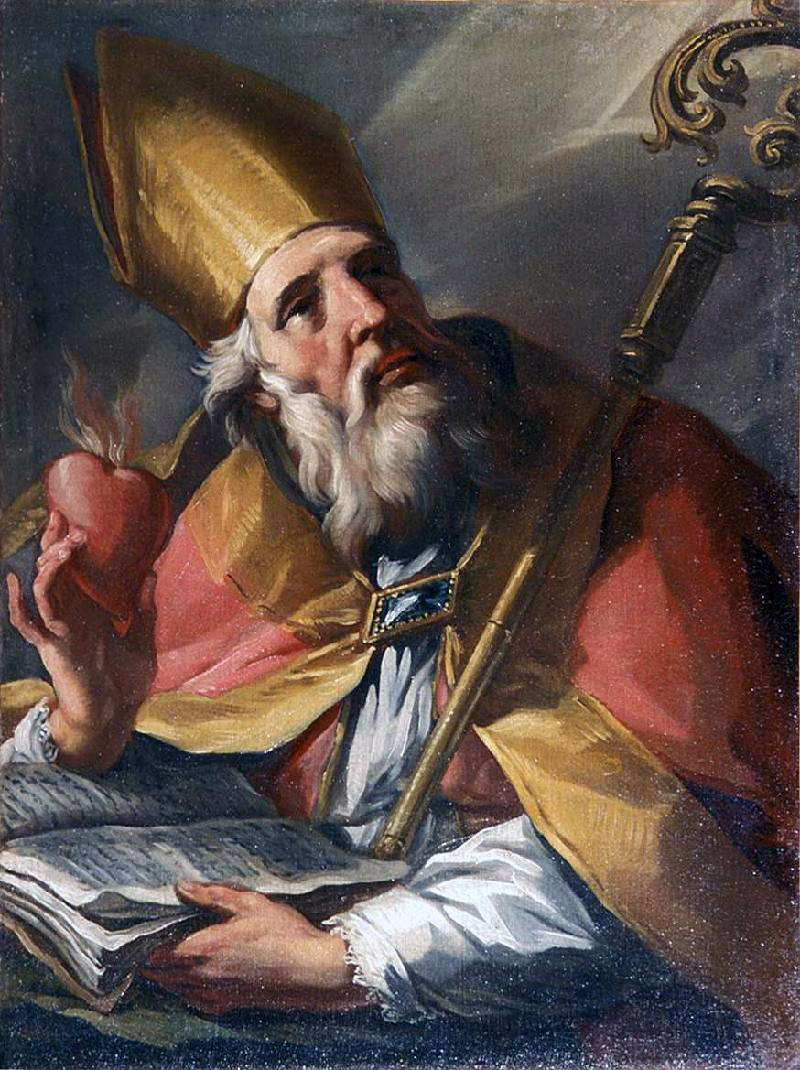
\includegraphics[width=0.5\textwidth]{ud-03/SanAgustin.jpg}
%\caption{San Agustín canonizado.\\
%(Fonte: wikimedia commons)}
%\label{fig:San-Agustin}
%\end{figure}
%
\begin{Figura}
  \centering
  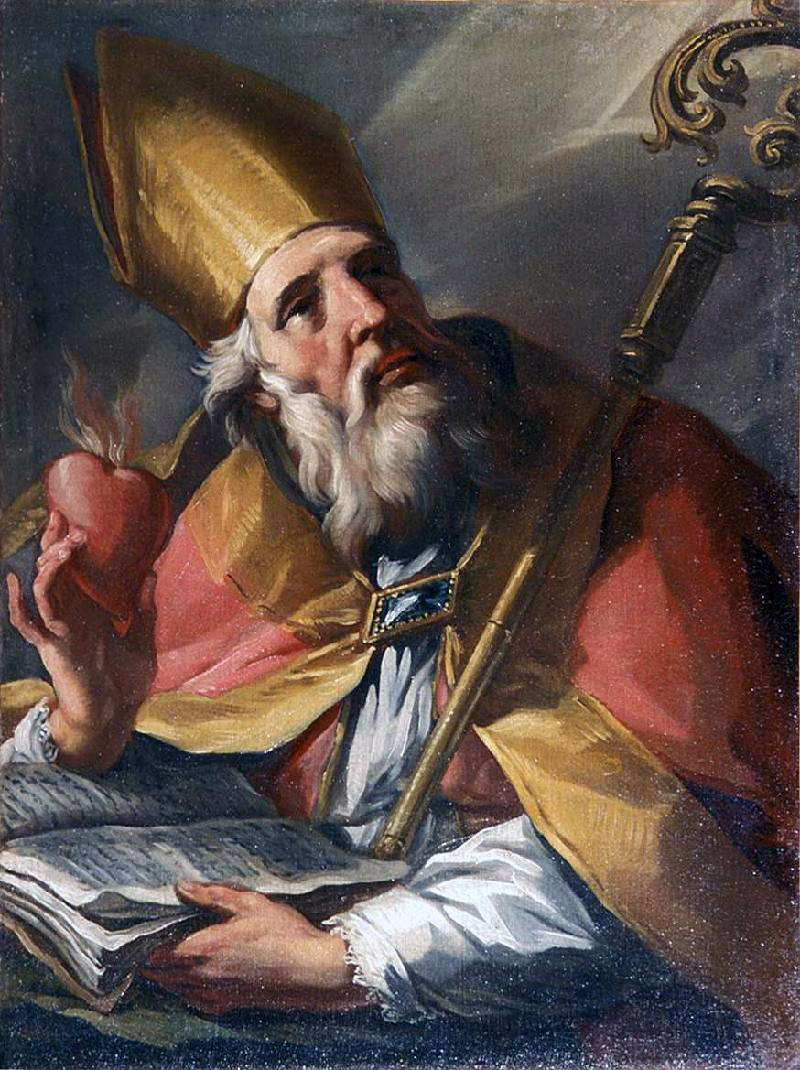
\includegraphics[width=0.75\textwidth]{ud-03/SanAgustin.jpg}
  \captionof{figure}{San Agustín canonizado.\\
  (Fonte: wikimedia commons)}
  \label{fig:San-Agustin}
\end{Figura}
%
\end{multicols}
%
\begin{quote}
\small{
``Velaquí que El case che dá o ton da melodía a cantar: non vaias en busca
do texto, coma se puideses traducir en sons articulados un canto no que
Deus se recree. Canta no xúbilo. Cantar con arte a Deus consiste niso:
cantar no xúbilo. Que significa cantar no xúbilo? Comprender e non saber
explicar en palabras o que se canta co corazón. Aqueles que cantan
durante a sega, ou durante a vendima, ou durante calquera outro
traballo, primeiro advirten o pracer que suscita o texto dos cantos,
pero máis tarde, cando a emoción crece, senten que non poden expresala
en palabras e entón desafóganse nunha soa modulación de notas. Este
canto denominámolo xúbilo.\\
O xúbilo é esa melodía coa que o corazón expresa todo o que non pode
expresar con palabras. E a quen elevar este canto senón a Deus? En
efecto, El é o que ti non podes expresar. E se non o podes expresar e
tampouco calalo, que outra cousa podes facer máis que xubilar? Entón o
corazón abrirase á alegría, sen utilizar palabras, e a grandeza
extraordinaria da alegría non coñecerá os límites das sílabas.
Cantádelle con arte no xúbilo.''
}
\end{quote}
%
\begin{ejercicio}[Pensamento musical Idade Media]
  \begin{enumerate}[1.-]
  \item
    En que época das que coñeces da Idade Media desenvolve as súas ideas sobre a música San Agustín? \ldots
%    \vspace*{0.5cm}
  \item
    Sinala no texto as palabras que fan referencia á concepción sobre música de San Agustín. \\
    Que cres que é para o autor ``cantar con xúbilo''? Consideras que está 
a favor ou en contra do uso do canto na Igrexa? Xustifica a túa resposta.
    \vspace*{3.10cm}
  \end{enumerate}
\end{ejercicio}
